\documentclass[twocolumn,a4paper,dvipdfmx]{ieicejsp}
\usepackage[T1]{fontenc}
\usepackage{lmodern}
\usepackage{textcomp}
\usepackage{latexsym}
\usepackage{float}
\usepackage{graphicx}
\usepackage{amsmath, amssymb}
\usepackage{bm}
\usepackage{upgreek}
\usepackage{caption}
\usepackage{booktabs}
\usepackage{multirow}
\usepackage{array}
\usepackage{tikz}
\usetikzlibrary{positioning, arrows.meta, fit}

\captionsetup{font=small}
\setlength{\floatsep}{12pt plus 2pt minus 2pt}
\setlength{\textfloatsep}{14pt plus 2pt minus 2pt}
\setlength{\dblfloatsep}{12pt plus 2pt minus 2pt}
\setlength{\dbltextfloatsep}{14pt plus 2pt minus 2pt}
\setlength{\intextsep}{12pt plus 2pt minus 2pt}

\title{
    {\bf 大喜利の回答文（ボケ）の構造ラベルの設計と視覚言語モデルによる自動判定}
    {\normalsize \\ Designing Structural Labels for Ogiri Responses and Their Automatic Annotation with Vision-Language Models}
}
\author{
    山富 龍 \\ Ryo Yamatomi
}
\affliate{%
    湘南工科大学 大学院 \\
    Graduate University of Shonan Institute of Technology\\
}

\begin{document}
\maketitle
\thispagestyle{plain}
\pagestyle{plain}

\begin{abstract}
大喜利投稿サイト「ボケて」に蓄積された約9,250万件の回答文（ボケ）を，大喜利の生成や判定の研究に用いるため，ボケの構造を表すラベルを設計し，自動で付与する方法を検討した．
実例の読解から，お題の形式が課す制約，ボケが誰の視点の言葉であるかを表す発話の型，面白さの理解に画像の外の知識が必要かの3つの観点を定め，定義書を3回改訂した．
検証データ620件の目視ラベルを作成し，同一の判断者が時間を置いて付け直したときの一致度を測ったところ，発話の型の6区分でマクロ F1 0.80，画像外の知識で F1 0.85 であり，これが自動判定の実質的な上限であることを示した．
カルタの制約の順守は書き出しの規則で，穴埋めとお題文の制約の順守は同じお題の他のボケとの類似度で判定でき，後者は付け替えた組との判別で AUC 0.81 を得た．
視覚言語モデル (Vision-Language Model，VLM) の教師とそのラベルで学習した文の埋め込みの分類器を比較した後，お題画像とボケを入力とする小さな VLM を教師ラベルで学習し，さらに少量の目視ラベルで微調整する二段階の学習を提案した．
この方法により，最終評価用データで発話の型の6区分のマクロ F1 を0.53から0.71〜0.74へ，画像外の知識の F1 を0.32から0.68〜0.70へ改善した．
さらに，同じお題のボケで共通する画像とお題の部分の計算をキャッシュとして共有することで，予測をほぼ変えずに推論を約4倍に高速化し，全件の処理時間の見積もりを約32日から約8日に短縮した．
\par
\noindent
{\bf キーワード} 大喜利，ユーモア，データアノテーション，視覚言語モデル，ラベル設計
\end{abstract}

\section*{Abstract}
To use about 92.5 million Ogiri responses (boke) collected from the Japanese comedy site Bokete for research on humor generation and evaluation, we designed labels that describe the structure of a boke and studied how to assign them automatically.
From close reading of real examples, we defined three aspects: compliance with the constraint imposed by the prompt format, the voice of the boke (whose words they are), and whether understanding the joke requires knowledge outside the image, and revised the guideline three times.
We built a validation set of 620 manually labeled boke and measured the agreement when the same annotator relabeled it later; the agreement was a macro F1 of 0.80 for the six voice classes and an F1 of 0.85 for outside knowledge, which we regard as a practical upper bound for automatic labeling.
Compliance with karuta prompts can be checked with a rule on the first character, and compliance with fill-in-the-blank and question prompts can be scored by similarity to other boke for the same prompt, achieving an AUC of 0.81 against swapped pairs.
After comparing vision-language model (VLM) teachers and text-embedding students distilled from them, we propose a two-stage training of small VLMs that take both the prompt image and the boke: training on teacher labels followed by fine-tuning on a small number of manual labels.
On the test set, this improves the macro F1 of the six voice classes from 0.53 to 0.71--0.74 and the F1 of outside knowledge from 0.32 to 0.68--0.70.
Finally, by sharing the cached computation of the image and prompt among the boke of the same prompt, we speed up inference about four times with nearly identical predictions, reducing the estimated time for all boke from about 32 days to about 8 days.
\par
\noindent
{\bf Key words} Ogiri, Humor, Data Annotation, Vision-Language Model, Label Design

\section{はじめに}
\label{sec_intro}
大喜利は，出題された題目に対して機知に富んだ回答を返す言葉遊びであり，ユーモアの生成と理解を扱う研究の題材として用いられている\cite{ref_oogiri_go, ref_newyorker}．
大喜利投稿サイト「ボケて」\cite{ref_bokete}では，投稿者がお題となる画像を掲示し，他の利用者がその画像に対する面白い一言を投稿する．
以下では，お題となる画像をお題画像，投稿された一言をボケと呼ぶ．
ボケてから収集したデータベースには，約682万件のお題画像と約9,250万件のボケが含まれる．
筆者らはこれまでに，全てのお題画像に大喜利の形式や画像の媒体を表すラベルを付与した．
本稿では，その次の段階として，ボケそのものにラベルを付与する方法を扱う．

ボケの生成や面白さの判定を学習・評価する際には，ボケがどのような作りの文であるかを知る必要がある．
例えば，画像の人物のセリフとして書かれたボケと，画像に題名を付けたボケでは，生成の際に与えるべき条件が異なる．
また，テレビ番組や歌の知識を前提とするボケは，その知識を持たないモデルには面白さを判断できない．
このようなボケを区別せずに評価すると，知識の不足による誤りとユーモアの理解の誤りを分けられない．
さらに，カルタのお題で札のひらがなから始まらないボケや，お題と無関係な書き込みは，生成の学習データから除くべきである．
したがって，ボケの作りを表すラベルを全てのボケに付与できれば，学習データの絞り込み，生成の条件付け，判定の誤りの分析に利用できる．

しかし，ボケのラベルには，お題画像のラベルにない2つの難しさがある．
第一に，何をラベルとすべきかが自明ではない．
ボケの区分には，笑いの手法や面白さのように主観的なものも多く，人でも判断が揃いにくい．
第二に，対象が約9,250万件と多い．
視覚言語モデル (Vision-Language Model，VLM) は画像と指示文から分類を行えるが，大規模なモデルを全件に適用すると，単一の GPU で数百日を要する．
本研究では，有料の API を用いず，単一の GPU で全件を現実的な時間で処理できる方法を目標とした．

本稿は，ラベルの設計から自動判定の方法の確立までの試行錯誤の経緯を，実験の結果とともに報告する．
主な内容は次のとおりである．
\begin{itemize}
    \item 実例の読解から，お題の形式が課す制約の順守，発話の型，画像外の知識の3つの観点を定め，定義書を3回改訂した経緯と，その判断の根拠を示す．
    \item 検証データ620件を作成し，同一の判断者による付け直しの一致度を測ることで，自動判定の精度の実質的な上限を示す．
    \item 制約の順守を，規則と同じお題の他のボケとの類似度で判定できることを示す．
    \item VLM の教師への指示，教師ラベルによる文の埋め込みの分類器，小さな VLM の微調整を比較し，教師ラベルと少量の目視ラベルによる二段階の学習が最も有効であることを示す．
    \item 画像外の知識の判定を改善するための試みと，その限界を示す．
    \item 同じお題のボケで計算を共有する推論の高速化を示す．
\end{itemize}

本稿の構成は次のとおりである．
\ref{sec_data}章で対象のデータと用語を定義し，\ref{sec_related}章で関連研究を整理する．
\ref{sec_label}章でラベルの設計の経緯を，\ref{sec_validation}章で検証データとその再現性を述べる．
\ref{sec_compliance}章で制約の順守の判定を，\ref{sec_text}章で VLM の教師と文の埋め込みの分類器による判定を述べる．
\ref{sec_vlm}章で小さな VLM の二段階の学習を，\ref{sec_outside}章で画像外の知識の改善の試みを述べ，\ref{sec_speed}章で推論の高速化を示す．
\ref{sec_discussion}章で得られた知見と限界を考察し，\ref{sec_conclusion}章でまとめる．

\section{対象のデータと用語}
\label{sec_data}
本研究で用いるデータベースは，ボケてから収集したお題画像6,823,270件と，それらに投稿されたボケ約9,250万件からなる．
ボケには，本文のほかに，お題の ID，投稿者，評価の合計（星の数）などの情報が含まれる．
サイトには不適切な投稿を示す \texttt{unsafe} と笑いの分類を示す \texttt{category} の項目もあるが，予備調査では \texttt{unsafe} はボケの0.03\%にしか付いておらず，\texttt{category} は89\%が既定値であったため，ラベルとしては用いなかった．
また，評価が5件以上付いたボケは全体の2〜4\%にとどまり，評価のないボケの多くは面白くないのではなく閲覧されていないと考えられる．

各お題画像には，筆者らの先行の作業により，大喜利の形式，画像中の文字の有無，画像の媒体，写真の簡潔な説明文（キャプション）が付与されている．
大喜利の形式は次の4つである．
\begin{itemize}
    \item 通常：画像に自由に一言を付ける．
    \item カルタ：画像の隅に書かれたひらがな1文字（札のかな）から始まる一言を答える．
    \item 穴埋め：画像中の文の空欄に入る語句を答える．
    \item お題文：画像に書かれた問いや指示に答える．
\end{itemize}
画像の媒体は，写真，アニメ，ゲーム，漫画，文字主体の画像，絵画，イラストの7つであり，複数を同時に持ちうる．
キャプションは写真にのみ付与されており，人物の名前は書かない設計である．
本稿では，これらをお題のラベルと呼び，ボケのラベルを推定する際の入力として用いる．

ボケの長さは形式によって異なる．
形式と媒体で分けた7つの層（\ref{sec_label}章）から300件ずつ抽出したお題の全てのボケ（約2.9万件）では，文字数の中央値は穴埋めが8，お題文が10，カルタが12，通常が14〜16であった．
穴埋めのボケは空欄に入る語だけのことが多く，お題画像の文と合わせなければ意味が分からない．

本稿では，Qwen3-VL-32B のように大規模な VLM を教師，教師が付けたラベル（教師ラベル）で学習する高速な分類器を生徒と呼ぶ．
目視ラベルは，画像とボケを表示して内容を確認できる AI エージェントである Claude Code が，その時点の定義書に従って付与した．
付与の際は，お題画像とボケを8組程度ずつ並べた一覧画像を作成し，評価する手法の予測は表示しなかった．
目視ラベルは全て同一の判断者によるものであり，複数の判断者の間の一致度は測っていない．
この点は本研究の限界であり，\ref{sec_discussion}章で改めて述べる．

\section{関連研究}
\label{sec_related}
\subsection{大喜利とユーモアの研究}
大喜利を対象とした研究として，Zhong らは画像やテキストのお題に対する大喜利の回答を集めたデータセット Oogiri-GO を構築し，大規模言語モデルによるユーモアの生成を評価した\cite{ref_oogiri_go}．
Hessel らは，風刺漫画のキャプションのコンテストのデータを用い，ユーモアの理解を，キャプションと漫画の対応付け，順位付け，説明の3つの課題として評価した\cite{ref_newyorker}．
これらの研究は回答の面白さを主な対象としており，回答がどのような作りの文であるかを表すラベルは扱っていない．
本研究は，面白さそのものではなく，回答の構造（制約の順守，発話の型，前提とする知識）を，生成や判定の条件や分析の軸として付与することを目的とする．

\subsection{視覚言語モデルと知識蒸留}
近年の VLM は，画像と指示文を入力として，指示に従った回答を学習なしで生成できる．
本研究では，Qwen3-VL\cite{ref_qwen3vl}，InternVL3.5\cite{ref_internvl35}，Gemma 3\cite{ref_gemma3}，SmolVLM\cite{ref_smolvlm}，LFM2-VL\cite{ref_lfm2vl}の公開モデルを比較した．
大規模なモデルの推論には vLLM\cite{ref_vllm}を用いた．
大規模なモデル（教師）の出力を小さなモデル（生徒）に学習させる知識蒸留\cite{ref_kd}は，推論の費用を下げる一般的な方法である．
本研究では，教師ラベルで学習した後に少量の目視ラベルで微調整する二段階の学習を用いる．
これは，教師ラベルの誤りを目視ラベルで補正する点で，ラベルの雑音を含む学習\cite{ref_noisy_student}と関係する．
大規模なモデルの微調整には，低ランクの行列を追加して学習する LoRA\cite{ref_lora}を用いた．
文の埋め込みには，日本語の文埋め込みモデル ruri-v3\cite{ref_ruri}と多言語の multilingual-e5\cite{ref_me5}を用いた．

\subsection{推論の高速化}
言語モデルの推論では，入力の先頭部分（プレフィックス）が共通する複数の要求の間で，注意機構のキーと値（KV キャッシュ）を共有することで計算を省く方法が用いられている\cite{ref_vllm, ref_sglang}．
本研究では，同じお題画像に投稿されたボケが，画像とお題の部分を共通のプレフィックスとして持つことに着目し，分類器の推論にこの考え方を適用する．

\section{ラベルの設計}
\label{sec_label}
ボケに付与するラベルは，最初から決まっていたわけではなく，実例の読解，試験的な分類，自動判定の結果を踏まえて段階的に改訂した．
本章では，その経緯と最終の定義を述べる．

\subsection{実例の読解と試験的な分類}
最初に，ボケのラベルとして「画像中のオブジェクトの知識に基づくか否か」「カルタの制約」「お題文への応答」「画像中の文字に基づくか」の4つの観点を候補とした．
これらが実際のボケに適用できるかを確かめるため，お題のラベルで7つの層を作り，層ごとに4件のお題を抽出した．
7つの層は，カルタ，穴埋め，お題文，通常の写真で文字を含むもの，通常の写真で文字を含まないもの，アニメまたは漫画を含むもの，それ以外の媒体である．
各お題から評価の上位3件と無作為の2件のボケを取り，計140件のボケをお題画像と並べて読んだ．
図\ref{fig_pilot}に一覧の例を示す．

\begin{figure}[t]
    \centering
    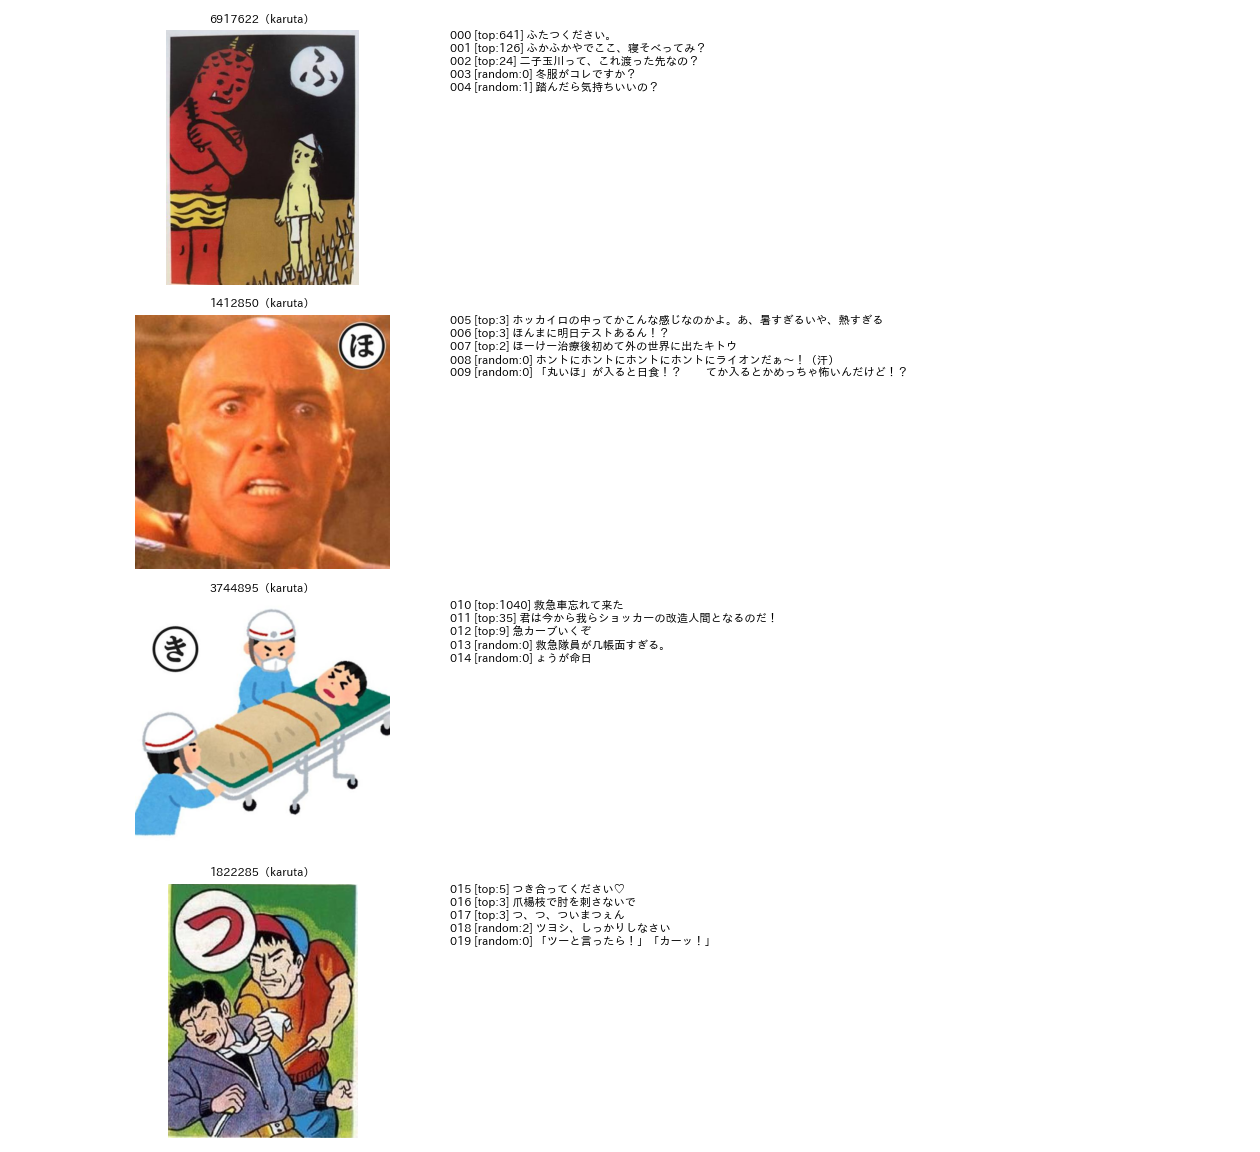
\includegraphics[width=\linewidth]{figures/fig_pilot_sheet.png}
    \caption{実例の読解に用いた一覧の例（カルタのお題）．左がお題画像，右がボケであり，top は評価の上位，random は無作為に選んだボケ，括弧内は評価の合計である．}
    \label{fig_pilot}
\end{figure}

読解の結果，候補の観点は性質の異なる2種類に分かれることが分かった．
一つは，お題の形式が課す制約である．
カルタの札のかなから始めることや，お題文の問いに答えることは，お題の形式でほぼ決まり，ボケに付けるべきなのは「制約に従っているか」だけである．
実際，かなで始まるボケが5件以上あるカルタのお題217件では，最も多い書き出しのかなの割合の中央値が0.91であり，制約はよく守られていた．
もう一つは，ボケの内容に関わる観点であり，こちらがボケ自体に付けるべき主なラベルである．

内容に関わる観点は，「知識に基づくか否か」の1軸では足りなかった．
140件に試験的に分類を付けたところ，知識の要らないボケは26\%にとどまり，一般常識が31\%，画像に写っていない番組・歌・CM・地域などの知識が31\%，画像に写る特定の人物やキャラクターの同定が11\%であった．
画像に写る対象の知識と，画像の外の文化や時事の知識では，生成でも判定でも必要な処理が異なるため，分けて扱う必要がある．
また，ボケは「誰の視点の，どのような言葉か」によって，セリフ，心の声，ツッコミ，状況の説明，名付け・見立て，回答に分かれた．
例えば，卓球選手が大きく反った写真には，「「起立」「気を付け」「ちょ礼」」のように画像の人物の掛け合いを書くボケと，「セルフ膝カックン！！！」のように画像に名前を付けるボケがあった．
以下では，この区分を発話の型と呼ぶ．
表\ref{tab_voice_examples}に，試験的な分類で見られた発話の型の例を，表\ref{tab_know_examples}に必要な知識の例を示す．

\begin{table}[t]
    \centering
    \caption{発話の型の例（試験的な分類より）．}
    \label{tab_voice_examples}
    \footnotesize
    \begin{tabular}{@{}p{0.27\linewidth}p{0.66\linewidth}@{}}
        \toprule
        型 & ボケの例 \\
        \midrule
        セリフ（S） & 「署長、こいつ下は隠さないのに顔は隠すんです。」 \\
        心の声（M） & 「男「どの秘密がバレたんだろう・・・」」 \\
        ツッコミ（T） & 「救急隊員が几帳面すぎる。」 \\
        状況の説明（N） & 「自宅でよさこいの練習をしていたらタンスの角に小指をぶつけた」 \\
        名付け・見立て（L） & 「異常な反応をしたリトマス紙」，「パステルのなめらかプリンを初めて食った時の俺」 \\
        回答（A） & 「サザエさん最終回のタイトルとは？」に「サザエンド」 \\
        \bottomrule
    \end{tabular}
\end{table}

\begin{table}[t]
    \centering
    \caption{必要な知識の4段階の例（試験的な分類より）．}
    \label{tab_know_examples}
    \footnotesize
    \begin{tabular}{@{}p{0.27\linewidth}p{0.66\linewidth}@{}}
        \toprule
        段階 & お題とボケの例 \\
        \midrule
        見た目だけ（0） & 赤ちゃんを抱いて寝る男性に「さ〜て。夜泣き開始。」 \\
        一般常識（G） & 「一石二鳥」の例えに「トイレ行ったら両方出た。」 \\
        画像中の対象（I） & ドラえもんのしずかちゃんのバイオリンに「バイオリン界のジャイアン」 \\
        画像外の事物（O） & チンパンジーの写真に「池の水抜いたらチンパンジー出てきた」（テレビ番組） \\
        \bottomrule
    \end{tabular}
\end{table}

\subsection{定義書の改訂}
試験的な分類を基に定義書を作成し，自動判定の結果と目視ラベルの見直しを踏まえて3回改訂した．
表\ref{tab_versions}に改訂の経緯を示す．

\begin{table}[t]
    \centering
    \caption{定義書の改訂の経緯．}
    \label{tab_versions}
    \small
    \begin{tabular}{@{}p{0.11\linewidth}p{0.47\linewidth}p{0.32\linewidth}@{}}
        \toprule
        版 & 主な内容 & 改訂の根拠 \\
        \midrule
        第1版 & 制約の順守，発話の型6区分，必要な知識4段階，画像中の文字への依存，性的・不適切の5項目 & 試験的な分類（140件） \\
        第2版 & 性的・不適切を削除．必要な知識を上から順に判定する手順とした & 不適切の自動判定が全ての方法で再現率0.27以下 \\
        第3版 & 必要な知識を画像外の知識の2値とし，条件と手順を厳密に定義．発話の型を判定の手順として定義し，3区分を併記 & 4段階の自動判定のマクロ F1 が0.48以下 \\
        \bottomrule
    \end{tabular}
\end{table}

第1版では，必要な知識を，見た目だけで分かる（0），一般常識（G），画像中のオブジェクトの情報（I），画像外のオブジェクト・事象の情報（O）の4段階とした．
当初は「画像に写る対象の同定」と呼んでいたが，固有名詞を言い当てられるかはモデルに依存するため，名前を言えるかではなく必要な情報の種類で判断するよう改めた．
また，お題文の「サザエさん」のように画像中の文字で名指しされた対象は，画像中のオブジェクトとした．

性的・不適切の項目は，検証データ（\ref{sec_validation}章）の6.4\%が該当したが，VLM の教師は性的なほのめかしの多くを見落とし，教師ラベルでの陽性率は0.9\%にとどまった．
その結果，教師ラベルで学習した分類器は陽性を1件も予測せず，最良の方法でも F1 0.42，再現率0.27にとどまった．
この項目は専用のデータを作らなければ扱えないと判断し，第2版で削除した．

必要な知識の4段階は，目視では上から順に判定すれば迷いが少なかった．
しかし，\ref{sec_text}章で述べるとおり，自動判定では4段階のマクロ F1 が最高でも0.48であり，見た目だけと一般常識の混同と，画像中と画像外の区別の難しさが残った．
一方，画像外の知識が要るか否かの2値は比較的安定して判定できた．
下流の生成や判定でも，外部の知識が要るボケを分けることが最も重要であるため，第3版では2値に改めた．

\subsection{最終の定義}
第3版の定義書は，次の4項目からなる．

\textbf{制約の順守}は，お題の形式が課す制約にボケが従っているかであり，はい，いいえ，対象外（通常の形式）の3値とする．
カルタは書き出しが札のかなと同じ音で始まるか，穴埋めは空欄に入る語句であるか，お題文は問いや指示に応じているかで判断する．
お題と無関係な書き込みは，形式によらず「いいえ」とする．

\textbf{発話の型}は，ボケが誰の視点の，どのような言葉であるかである．
6区分は，次の問いを順に確かめて決める．
\begin{enumerate}
    \item 形式が穴埋め・お題文で，ボケが空欄や問いへの答えであれば，回答（A）とする．
    \item ボケが名詞句で，画像全体や写っている物に名前・題・例えを付けていれば，名付け・見立て（L）とする．
    \item 話し手が画像の中の人物・動物・物であれば，声に出している言葉をセリフ（S），心の中の考えや独り言を心の声（M）とする．迷う場合はセリフとする．
    \item 話し手が画像の外の人であれば，画像の出来事や前後の状況を説明する文を状況の説明（N），画像を見て言う感想・指摘・ツッコミや画像の人物への呼びかけをツッコミ（T）とする．
\end{enumerate}
6区分は人でも判断が分かれやすいため，信頼性の低いラベルとして扱い，登場人物の言葉（S，M），外からの言葉（T，N，L），回答（A）の3区分を併記する．

\textbf{画像外の知識}は，面白さを理解するのに，画像にも画像中の文字にも示されていない特定の事物の知識が必要かであり，次の3条件を全て満たすときに「はい」とする．
\begin{enumerate}
    \item 特定性：依存する事物が，特定の作品・人物・商品・番組・歌・地名の印象・出来事・流行語・ネットの定型・有名な台詞・ボケての慣習などである．
    \item 画像の外：その事物が画像に写っておらず，画像中の文字でも名指しされていない．
    \item 必要性：その事物を知らないと面白さが成り立たない．
\end{enumerate}
一般の語彙，慣用句，ラジオ体操のように誰もが知る生活の事物，一般的な職業やジャンルの印象は「いいえ」とする．

\textbf{画像中の文字への依存}は，ボケの意味が画像中の文字を読まないと分からないかである．
この項目は形式でほぼ決まり，穴埋め・お題文は依存し，通常はほぼ依存しない．
第1版の検証データ（最終評価用210件）で，形式だけの規則で F1 0.77，\ref{sec_text}章で述べる目視ラベルによる補正で F1 0.90 が得られたため，以下では詳しく扱わない．

\section{検証データと目視ラベルの再現性}
\label{sec_validation}
\subsection{検証データの作成}
検証データは，定義書の改訂に合わせて2回に分けて作成した．
最初に，\ref{sec_label}章の7つの層から各12件のお題を抽出し，各お題から評価の上位3件と無作為の2件のボケを取って420件とした．
この420件では，セリフと回答が大半を占め，ツッコミは12件，心の声は28件しかなかった．
そこで，教師または規則が心の声，ツッコミ，状況の説明，名付け・見立て，セリフのいずれかと予測したボケから，型ごとに40件を予測を見せずに追加し，計620件とした．
ツッコミの候補は，教師も規則もツッコミと予測したボケであったが，目視では多くがセリフか状況の説明であり，追加後もツッコミは26件にとどまった．

620件は，お題の単位で層ごとに半数ずつ，調整用データ（dev，308件）と最終評価用データ（test，312件）に分けた．
指示文や構成の選択には調整用データだけを用い，最終評価用データは精度の報告にのみ用いた．
評価指標には，各クラスの F1 の平均であるマクロ F1 を用いた．
クラス $ k $ の適合率を $ P_k $，再現率を $ R_k $ とすると，マクロ F1 は(\ref{eq_macro_f1})で表される．

\begin{equation}
    {\rm F1}_{\rm macro} = \frac{1}{K} \sum_{k=1}^{K} \frac{2 P_k R_k}{P_k + R_k}
    \label{eq_macro_f1}
\end{equation}

\noindent
ここで $ K $ はクラス数である．
画像外の知識は2値であるため，「はい」のクラスの F1 を用いた．
最終評価用データの F1 の95\%信頼区間は，項目を復元抽出する1,000回のブートストラップで求めた．

\subsection{目視ラベルの見直し}
目視ラベルは同一の判断者によるものであり，判断の揺れや系統的な誤りを含みうる．
最初の420件では，2つの教師がともに目視と異なった項目を定義書に照らして見直した．
対象は必要な知識143件，発話の型109件，不適切19件であったが，大半は教師の系統的な偏りであり，定義書が教師を支持した38件だけを改めた．
第3版で必要な知識を2値に改めた際には，620件の全てを新しい定義で見直し，27件を改めた．
画像外の知識が「はい」の項目は620件中139件であった．

\subsection{付け直しによる再現性の測定}
自動判定の精度がどこまで上がりうるかを知るため，620件の全てを無作為に並べ替え，元の番号とラベルを伏せた一覧で，定義書 第3版に従って付け直した．
付け直しは，同じ判断者が時間を置いて行ったものであり，判断者の間の一致度ではなく，同一の判断者の再現性を表す．
表\ref{tab_reliability}に，元のラベルとの一致を示す．

\begin{table}[t]
    \centering
    \caption{元の目視ラベルと付け直したラベルの一致（620件）．$\kappa$ は Cohen の $\kappa$ 係数\cite{ref_kappa}である．}
    \label{tab_reliability}
    \small
    \begin{tabular}{lccc}
        \toprule
        項目 & F1 & 一致率 & $\kappa$ \\
        \midrule
        発話の型 6区分（マクロ） & 0.80 & 0.86 & 0.82 \\
        発話の型 3区分（マクロ） & 0.93 & --- & --- \\
        画像外の知識 & 0.85 & --- & 0.81 \\
        \bottomrule
    \end{tabular}
\end{table}

6区分のクラスごとの F1 は，回答が0.94，セリフが0.89，状況の説明が0.85，名付け・見立てが0.81である一方，心の声は0.75，ツッコミは0.55であった．
不一致で多かったのは，心の声とセリフ（11件），セリフとツッコミ，状況の説明と名付け・見立ての間の揺れであった．
また，形式が通常でも，お題画像に空欄や空の吹き出し，問いが含まれる場合に回答とするかの揺れが約10件あった．

不一致の項目は定義書に照らして裁定し，合意ラベルとした．
裁定では，お題画像が空欄・空の吹き出し・問いを課している場合は形式によらず回答とし，迷う場合はセリフとし，画像外の知識で判断が分かれた項目は元のラベルを維持した．
合意ラベルは元のラベルから，発話の型で55件，画像外の知識で22件が変わった．
以下の評価は，特に断らない限り，全ての方法をこの合意ラベルで評価し直した値である．
そのため，各実験の当時に報告した値とは小数第2位で異なる場合がある．

表\ref{tab_reliability}の一致度は，同じ定義でも時間を置くと6区分の約14\%の判断が変わり，少ないクラスほど揺れが大きいことを示す．
したがって，自動判定の F1 が6区分で0.8，画像外の知識で0.85を大きく超えることは期待しにくく，これらの値を実質的な上限とみなす．

\section{制約の順守の判定}
\label{sec_compliance}
\subsection{カルタ}
カルタの制約は，ボケの書き出しのかなと札のかなの一致で判定できる．
札のかなはお題のラベルに含まれないため，同じお題のボケの書き出しのかなの最頻値を札のかなとした．
漢字で始まるボケは pykakasi で読みに変換したが，「辛い」（からい，つらい）のように複数の読みがありうるため，漢字で始まるボケは順守とみなした．
第1版の検証データのカルタ・穴埋め・お題文のボケ90件で，この規則の正解率は0.97であり，違反4件のうち2件を検出した．
VLM の教師の正解率は0.88〜0.98であり，規則と同程度であったが，速度は規則の数千分の一であった．
カルタ以外の形式で制約に反するボケは，ほとんどが宣伝や他のボケへの返信などの無関係な書き込みであった．

\subsection{穴埋めとお題文}
穴埋めとお題文の制約は，文字の一致では確かめられず，ボケが空欄や問いに意味の上で応じているかを判断する必要がある．
しかし，実際の違反はまれであり，検証データの穴埋め・お題文のボケ120件では1件しかなかった．
そこで，検証データの穴埋め・お題文のボケを，同じ形式の別のお題に付け替えた組120件を違反の代わりとし，元の組120件との判別で方法を比較した．

比較した方法は，VLM の教師（Qwen3-VL-32B，30B-A3B）にお題画像とボケを与えて問う方法，ボケの文の埋め込みとお題画像の埋め込みを連結して正しい組と付け替えた組を判別する MLP（学習用に2万件の組を作成），同じお題の他のボケとの類似度の3種類である．
類似度は，ボケ $ b $ の文の埋め込みを $ {\mathbf e}_b $ とし，同じお題の他のボケ（最大50件）のうち $ {\mathbf e}_b $ と最も似た5件の集合を $ {\mathbb N}_5(b) $ として，(\ref{eq_knn})で求めた．

\begin{equation}
    s(b) = \frac{1}{5} \sum_{b' \in {\mathbb N}_5(b)} \cos ( {\mathbf e}_b, {\mathbf e}_{b'} )
    \label{eq_knn}
\end{equation}

\noindent
文の埋め込みには ruri-v3-310m\cite{ref_ruri}の平均プーリングを用いた．
同じお題の他のボケは「お題が求める答えの方向」を表すため，お題の文を書き起こさなくても応答の妥当性を測れると考えた．
比較のため，最も似た5件ではなく他のボケ全ての埋め込みの平均とのコサイン類似度も求めた．

表\ref{tab_compliance}に結果を示す．
検出率は，正しい組の95\%を順守と判定するしきい値で，付け替えた組を検出できた割合である．

\begin{table}[t]
    \centering
    \caption{穴埋め・お題文の制約の順守の判別（正120組，付け替え120組）．}
    \label{tab_compliance}
    \small
    \begin{tabular}{lcccc}
        \toprule
        方法 & AUC & 検出率 & 穴埋め & お題文 \\
        \midrule
        教師 32B & 0.55 & 13\% & --- & --- \\
        教師 30B-A3B & 0.52 & 6\% & --- & --- \\
        組の分類器 & 0.57 & 10\% & 0.54 & 0.65 \\
        他のボケの平均 & 0.75 & 32\% & 0.66 & 0.83 \\
        類似度 $ s(b) $ & \textbf{0.81} & \textbf{39\%} & \textbf{0.73} & \textbf{0.88} \\
        \bottomrule
    \end{tabular}
\end{table}

VLM の教師は，付け替えた組もほぼ全て順守と判定し，画像の空欄や問いとボケの対応を確かめられなかった．
組の分類器も弱く，画像全体の埋め込みはお題の文の中身を表さないと考えられる．
同じお題の他のボケとの類似度が最も良く，特に最も似た5件との類似度は，典型から外れた正しいボケも拾える点で平均との類似度を上回った．
お題文では AUC 0.88 であったのに対し，穴埋めでは空欄に入る語がボケどうしで多様なため0.73にとどまった．

この得点は他のボケと似ているかを測るため，意外性のある正しいボケも低くなりうる．
そこで，しきい値で二分せず得点のまま付与し，生成の学習データから下位数\%を除く用途や，判定の特徴として用いることを提案する．
また，ボケの少ないお題では計算できないため，その場合にはお題の文の書き起こしが必要になる．

\section{VLM の教師と文の埋め込みの生徒}
\label{sec_text}
本章では，発話の型と必要な知識について，規則，VLM の教師，教師ラベルで学習した文の埋め込みの分類器（生徒）を比較した経緯を述べる．

\subsection{第1版での比較}
最初の比較では，第1版の検証データ420件（最終評価用210件，当時の目視ラベル）を用いた．
規則は，形式が穴埋め・お題文なら回答とし，それ以外は括弧，文末，呼びかけの語などの手がかりで発話の型を決めた．
教師は Qwen3-VL の 8B，30B-A3B，32B であり，お題画像，形式，ボケを与えて全項目を JSON で答えさせた．
生徒は，30B-A3B が学習用のボケ3.5万件に付けたラベルで学習した MLP であり，入力はボケの文の埋め込み，お題の形式・属性・媒体，お題画像の埋め込みの組み合わせとした．

表\ref{tab_v1}に，最終評価用210件での結果を示す．

\begin{table}[t]
    \centering
    \caption{第1版の検証データ（最終評価用210件，当時の目視ラベル）での比較．発話の型と必要な知識はマクロ F1，文字は画像中の文字への依存の F1，順守はカルタ・穴埋め・お題文のボケの正解率，速度は1秒あたりの件数．第2版は教師への指示の改訂版である．生徒は3 seed の平均．}
    \label{tab_v1}
    \footnotesize
    \setlength{\tabcolsep}{2.5pt}
    \begin{tabular}{@{}lccccr@{}}
        \toprule
        方法 & 発話 & 知識 & 文字 & 順守 & 速度 \\
        \midrule
        規則 & 0.45 & 0.12 & 0.77 & \textbf{0.97} & 約4.1万 \\
        教師 8B（第1版） & 0.41 & 0.32 & 0.70 & 0.88 & 11 \\
        教師 30B-A3B（第1版） & 0.47 & 0.15 & 0.71 & 0.98 & 14 \\
        教師 30B-A3B（第2版） & 0.41 & 0.47 & 0.78 & 0.97 & 12 \\
        教師 32B（第1版） & 0.53 & 0.29 & 0.75 & 0.98 & 6 \\
        教師 32B（第2版） & \textbf{0.56} & 0.43 & 0.74 & 0.96 & 4 \\
        生徒 MLP（文） & 0.23 & 0.35 & 0.52 & 0.97 & 約40万 \\
        生徒 MLP（文＋形式） & 0.33 & 0.39 & 0.77 & 0.97 & 約40万 \\
        生徒 MLP（文＋形式＋画像） & 0.36 & 0.36 & 0.77 & 0.97 & 約39万 \\
        生徒 文の分類器の微調整 & 0.39 & 0.42 & 0.78 & 0.97 & 約3,100 \\
        目視ラベルのみ（210件） & 0.37 & 0.36 & \textbf{0.90} & 0.82 & --- \\
        生徒＋目視ラベルで補正 & 0.42 & \textbf{0.48} & \textbf{0.90} & 0.89 & --- \\
        \bottomrule
    \end{tabular}
\end{table}

この段階では，発話の型の6区分のマクロ F1 は規則が0.45，32B が0.56であり，生徒は0.23〜0.39と規則を下回った．
生徒の速度は文の埋め込みの計算を含まない値であり，埋め込みは約4,700〜9,600件/秒で計算できた．
主な原因は教師の偏りであった．
30B-A3B は学習用のボケの48\%をツッコミとし，状況の説明をほとんど付けなかったため，生徒はこの偏りを受け継いだ．
必要な知識の4段階のマクロ F1 は最高でも0.48であった．
教師は「急カーブ」「つきあい」のような一般的な語を特定の事物とし，30B-A3B は第1版の指示で知識をほぼ全て画像中のオブジェクトとした．
一方，最終評価用210件の目視ラベルで生徒の出力を補正すると（以下，補正），必要な知識と画像中の文字の精度が教師と同等以上になり，少量の目視ラベルの効果が大きいことが示された．
補正では，生徒の出力の確率とお題の特徴を入力とするロジスティック回帰を，調整用データの目視ラベルで学習して最終評価用データを予測し，逆の組み合わせも行った．

\subsection{教師ラベルの水増しと重み付き損失}
発話の型の生徒を改善するため，最も精度の高い 32B の教師で，学習用のボケ9,041件にラベルを付け直した．
内訳は，無作為の5,000件と，規則か教師が少ない型と予測した候補の約4,000件である．
さらに，型の出現回数の逆数で重みを付けた交差エントロピーで学習した．
表\ref{tab_text_students}に，検証データ620件の合意ラベルで評価した結果を示す．

\begin{table}[t]
    \centering
    \caption{規則，教師，文の埋め込みの生徒の比較（合意ラベル）．6区分と3区分はマクロ F1，画像外は「はい」の F1．生徒は3 seed の平均である．}
    \label{tab_text_students}
    \small
    \begin{tabular}{@{}lcccc@{}}
        \toprule
        & \multicolumn{2}{c}{6区分} & 3区分 & 画像外 \\
        方法 & dev & test & test & test \\
        \midrule
        規則 & 0.49 & 0.51 & 0.74 & --- \\
        教師 32B（第3版） & 0.49 & 0.53 & 0.81 & 0.32 \\
        教師 30B-A3B（第3版） & 0.44 & 0.41 & 0.72 & 0.47 \\
        生徒（水増し＋重み） & 0.54 & 0.56 & 0.81 & 0.14 \\
        生徒（水増し＋重み＋補正） & 0.58 & 0.61 & 0.81 & 0.47 \\
        教師 32B（one\_kt\_cap） & 0.56 & 0.56 & 0.79 & \textbf{0.67} \\
        生徒（one\_kt\_cap，3.5万件） & \textbf{0.65} & \textbf{0.61} & \textbf{0.82} & 0.60 \\
        \bottomrule
    \end{tabular}
\end{table}

水増しと重み付き損失により，生徒の6区分は教師を上回った．
生徒は画像を入力せず文と形式だけを用いるが，教師が状況の説明をほとんど使わない偏りを重み付き損失が打ち消したためと考えられる．
一方，ツッコミはどの方法でも F1 0.2前後であった．
教師はツッコミを多用し，水増し用の集合の33\%をツッコミとしたのに対し，目視では検証データの4\%しかない．

6区分のうち，セリフと心の声を統合した5区分ではマクロ F1 が最高0.66，さらにツッコミ・状況の説明・名付け・見立てを外からの言葉に統合した3区分では0.82であった（当時の目視ラベル）．
この結果を受けて，第3版では6区分を信頼性の低いラベルとし，3区分を併記した．

\subsection{必要な知識の判定の試み}
必要な知識の4段階を改善するため，第2版では，見た目だけで分かるか，一般常識を加えれば分かるか，画像中の対象の情報が要るか，画像外の情報が要るかを順に問う指示を教師に与えた．
しかし，順に問うと最初の問いに真と答えやすくなり，見た目だけに偏ったため，4段階のマクロ F1 は32B で0.42，30B-A3B で0.37にとどまった．
また，固有名詞の割合などの品詞の特徴34次元を形態素解析で作り，生徒の入力に加えたが，効果はなかった．
固有名詞を含まない有名な台詞の引用や，固有名詞を含んでも画像中の対象の名前であるボケが多いことと，形態素解析の辞書が漫画やタレントの名前を固有名詞と判定しないことが原因であった．
表\ref{tab_text_students}の教師 32B（第3版）の画像外の F1 は，この順に問う指示で「画像外」と判定された項目を「はい」とみなした値であり，再現率が低い．

\subsection{教師の指示の比較}
第3版の定義に合わせて，32B の教師への指示を6通りに書き直し，調整用データで比較した．
6通りは，第3版の手順を示して6区分から1つを選ばせ，画像外の知識を1つの真偽で問う指示（one），one に写真のキャプションと媒体・文字の有無を文で加えた指示（one\_cap），one\_cap の画像外の知識の問いを，依存する事物とその種類（作品，人物，商品，地名，出来事，ボケての慣習，一般，なし）を選ばせる問いに替えた指示（one\_kt\_cap），発話の型を話し手・名付けか・声に出すか・説明かの別の問いに分解し規則で6区分にする指示（dec），dec に13の例を加えた指示（dec\_fs）である．
図\ref{fig_teacher_prompts}に結果を示す．

\begin{figure}[t]
    \centering
    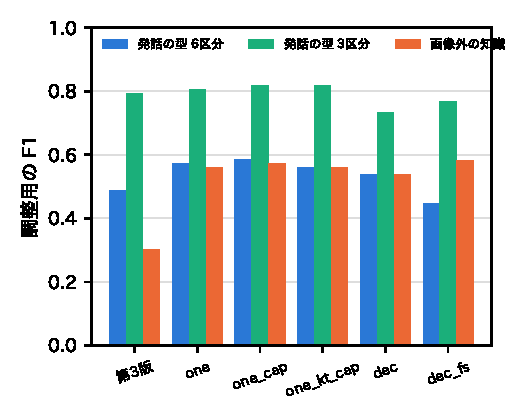
\includegraphics[width=\linewidth]{figures/fig_teacher_prompts.pdf}
    \caption{教師（Qwen3-VL-32B）の指示ごとの調整用データでの F1（合意ラベル）．第3版は4段階を順に問う指示，他は第3版の定義に合わせて書き直した指示である．}
    \label{fig_teacher_prompts}
\end{figure}

手順を書き込んで1つを選ばせる one は，第3版の指示より6区分が0.49から0.57に上がり，キャプションを加えた one\_cap で0.58となった．
一方，問いの分解は6区分をかえって下げた．
分解した指示では，モデルが話し手を「画像を見ている人」と答える偏りがあり，セリフ211件のうち134件がツッコミになった．
話し手の既定を画像の中の誰かとするよう問い直しても，最終評価用では one に及ばなかった．
例示も発話の型をツッコミに寄せた．
画像外の知識では，依存する事物の種類を選ばせる one\_kt\_cap が，普通名詞を特定の事物とする誤りを減らし，最終評価用で F1 0.67と最も高かった．
以上から，教師は one\_kt\_cap とし，学習用のボケ3.5万件（水増し用の9,041件と，他の学習用のボケ25,593件）に付け直した．
このラベルで学習した文の生徒は，6区分で調整用0.65，最終評価用0.61，画像外の知識で0.60となった．

文の生徒は，文の埋め込みの計算を含めても全件を短時間で処理できる．
しかし，画像外の知識では教師との差が大きく，画像に写っている対象と画像外の事物を区別するには画像の情報が要ると考えられた．
次章では，お題画像とボケの両方を入力とする VLM を生徒とする．

\section{小さな VLM の二段階の学習}
\label{sec_vlm}
\subsection{分類器の構成}
お題画像とボケの両方を入力とする生徒として，1〜8B の VLM を分類器にした．
VLM に，お題画像と「大喜利サイト「ボケて」のお題画像（形式：$ \cdot $）に投稿されたボケ：「$ \cdot $」」という文を入力し，言語モデルの最終層の，入力の最後のトークンの隠れ状態 $ {\mathbf h} \in {\mathbb R}^{H} $ を取り出す．
発話の型の確率 $ {\mathbf p} \in {\mathbb R}^{6} $ と画像外の知識の確率 $ q $ を，(\ref{eq_heads})で求める．

\begin{align}
    {\mathbf p} &= {\rm softmax} ( {\mathbf W}_{\rm v} {\mathbf h} + {\mathbf b}_{\rm v} ) \nonumber \\
    q &= \sigma ( {\mathbf w}_{\rm o}^{\top} {\mathbf h} + b_{\rm o} )
    \label{eq_heads}
\end{align}

\noindent
ここで $ {\mathbf W}_{\rm v} \in {\mathbb R}^{6 \times H} $，$ {\mathbf b}_{\rm v} \in {\mathbb R}^{6} $，$ {\mathbf w}_{\rm o} \in {\mathbb R}^{H} $，$ b_{\rm o} \in {\mathbb R} $ は出力層のパラメータ，$ \sigma $ はシグモイド関数，$ H $ は隠れ状態の次元数である．
生成を行わず1回の順伝播で判定するため，VLM に回答を生成させる場合より速い．
VLM の全ての線形層にランク16の LoRA\cite{ref_lora}を付けて学習した．
お題画像は長辺448画素以下に縮小し，タイル分割を止めて画像のトークン数を200〜300程度にそろえた．

損失は，発話の型の正解 $ y $ と画像外の知識の正解 $ t \in \{0, 1\} $ に対し，(\ref{eq_loss})とした．

\begin{equation}
    {\mathcal L} = - \alpha_{y} \log p_{y} - \lambda \left\{ \beta \, t \log q + (1 - t) \log (1 - q) \right\}
    \label{eq_loss}
\end{equation}

\noindent
ここで $ \alpha_{y} $ は学習データでのクラス $ y $ の出現率の逆数の平方根に比例する重み，$ \beta $ は負例と正例の件数の比，$ \lambda $ は画像外の知識の損失の重み（\ref{sec_outside}章を除き $ \lambda = 1 $）である．
最適化には AdamW\cite{ref_adamw}を用い，LoRA の学習率を $ 10^{-4} $，出力層をその10倍とし，最初の5\%のステップで線形に増やした後に余弦関数で減衰させた．

\subsection{学習の手順}
学習は次の二段階で行った．
\begin{enumerate}
    \item 段階1：教師（32B，one\_kt\_cap）のラベル34,634件で，バッチサイズ16で1〜2エポック学習する．教師ラベルの1割を検証用に取り分けた．
    \item 段階2：段階1の重みから，学習用の目視ラベル931件で，バッチサイズ8，学習率 $ 5 \times 10^{-5} $ で4エポック微調整し，調整用データで最良のエポックを選ぶ．
\end{enumerate}
学習用の目視ラベル931件は，教師ラベルの集合（検証データのお題を含まない）から，お題1件につき1件まで抽出した．
半数は無作為に選び，残りは教師ラベルで少ない型（心の声，ツッコミ，状況の説明，名付け・見立て）と画像外の知識が「はい」のボケを多めに選んだ．
内訳は，セリフ248件，回答206件，状況の説明156件，名付け・見立て152件，心の声109件，ツッコミ60件であり，画像外の知識が「はい」は26\%であった．
この931件で教師ラベルと目視ラベルを比べると，6区分のマクロ F1 は0.65（ツッコミ0.33，状況の説明0.51），画像外の知識の F1 は0.63であり，教師ラベルには大きな誤りが含まれていた．

比較のため，指示だけで判定させる方法（ゼロショット）と，段階1を行わず目視ラベルだけで8エポック学習する方法も評価した．
ゼロショットでは，vLLM で one\_kt\_cap の指示を与えて JSON を生成させた．

\subsection{結果}
表\ref{tab_zeroshot}にゼロショットの結果を，表\ref{tab_vlm}に微調整の結果を，図\ref{fig_progress}に段階ごとの最終評価用データでの F1 を示す．

\begin{table}[t]
    \centering
    \caption{ゼロショットの比較（合意ラベル）．速度は vLLM で620件を一括で生成したときの1秒あたりの件数，形式は JSON を読み取れた割合．（推）は推論の後に回答する Thinking モデル．}
    \label{tab_zeroshot}
    \footnotesize
    \setlength{\tabcolsep}{1.8pt}
    \begin{tabular}{@{}lcccccc@{}}
        \toprule
        & \multicolumn{2}{c}{6区分} & 3区分 & 画像外 & & \\
        モデル & dev & test & test & test & 速度 & 形式 \\
        \midrule
        Qwen3-VL-2B & 0.28 & 0.28 & 0.54 & 0.44 & 11.7 & 1.00 \\
        Qwen3-VL-4B & 0.44 & 0.42 & 0.74 & 0.39 & 15.2 & 1.00 \\
        Qwen3-VL-8B & 0.44 & 0.41 & 0.71 & 0.56 & 11.9 & 1.00 \\
        InternVL3.5-1B & 0.30 & 0.30 & 0.56 & 0.00 & 13.5 & 1.00 \\
        InternVL3.5-2B & 0.25 & 0.29 & 0.56 & 0.00 & 11.5 & 1.00 \\
        InternVL3.5-4B & 0.30 & 0.32 & 0.67 & 0.00 & 7.3 & 1.00 \\
        LFM2-VL-1.6B & 0.29 & 0.28 & 0.64 & 0.00 & 24.8 & 0.99 \\
        LFM2-VL-3B & 0.30 & 0.26 & 0.56 & 0.07 & 19.0 & 1.00 \\
        SmolVLM2-2.2B & 0.25 & 0.26 & 0.58 & 0.00 & 5.1 & 1.00 \\
        Gemma 3 4B & 0.31 & 0.32 & 0.58 & 0.57 & 8.3 & 1.00 \\
        Qwen3-VL-30B-A3B（推） & 0.45 & 0.48 & 0.72 & 0.50 & 0.7 & 0.56 \\
        Qwen3-VL-32B（推） & \textbf{0.50} & \textbf{0.52} & \textbf{0.79} & \textbf{0.61} & 0.3 & 0.77 \\
        \bottomrule
    \end{tabular}
\end{table}

\begin{table}[t]
    \centering
    \caption{小さな VLM の微調整の比較（合意ラベル．dev は調整用，test は最終評価用）．速度は前処理を含む1秒あたりの件数（分類器の推論，バッチ32）．}
    \label{tab_vlm}
    \footnotesize
    \setlength{\tabcolsep}{3pt}
    \begin{tabular}{@{}lccccc@{}}
        \toprule
        & \multicolumn{2}{c}{6区分} & 3区分 & 画像外 & \\
        方法 & dev & test & test & test & 速度 \\
        \midrule
        \multicolumn{6}{@{}l}{段階1のみ（教師ラベル）} \\
        \quad Qwen3-VL-4B & 0.61 & 0.55 & 0.79 & 0.70 & 33 \\
        \quad InternVL3.5-2B & 0.58 & 0.57 & 0.79 & 0.66 & 46 \\
        \multicolumn{6}{@{}l}{目視ラベルのみ} \\
        \quad Qwen3-VL-4B & 0.69 & 0.67 & 0.84 & 0.55 & 33 \\
        \quad Qwen3-VL-2B & 0.69 & 0.71 & 0.86 & 0.55 & --- \\
        \multicolumn{6}{@{}l}{段階1＋段階2} \\
        \quad InternVL3.5-1B & 0.71 & 0.69 & 0.85 & 0.61 & --- \\
        \quad InternVL3.5-2B & \textbf{0.77} & 0.71 & 0.85 & 0.64 & 46 \\
        \quad InternVL3.5-4B & 0.72 & 0.71 & 0.85 & 0.67 & --- \\
        \quad Qwen3-VL-2B & 0.69 & 0.65 & 0.84 & 0.62 & --- \\
        \quad Qwen3-VL-4B & 0.76 & 0.71 & 0.86 & 0.69 & 33 \\
        \quad LFM2-VL-1.6B & 0.71 & 0.64 & 0.85 & 0.64 & --- \\
        \bottomrule
    \end{tabular}
\end{table}

\begin{figure}[t]
    \centering
    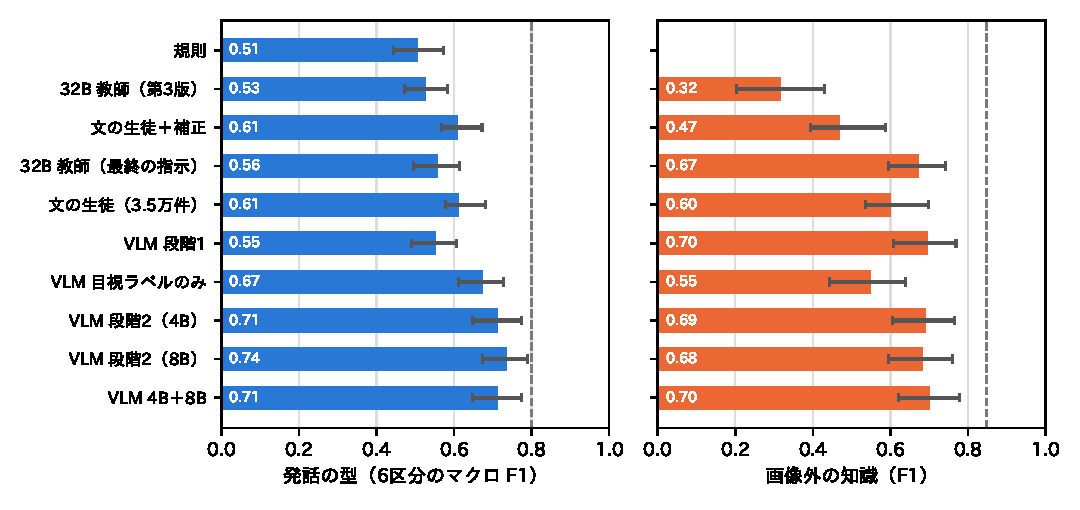
\includegraphics[width=\linewidth]{figures/fig_progress.pdf}
    \caption{主な段階の方法の最終評価用データ（312件）での F1 と95\%信頼区間．破線は目視ラベルの再現性（表\ref{tab_reliability}）．規則は画像外の知識を判定しない．}
    \label{fig_progress}
\end{figure}

ゼロショットでは，小さな VLM は指示だけでは判定できなかった．
6区分は最良の Qwen3-VL-4B でも0.42であり，InternVL3.5，LFM2-VL，SmolVLM2 は画像外の知識をほぼ全て「いいえ」とした．
推論を行う 32B の Thinking モデルも，6区分0.52，画像外の知識0.61で，教師（Instruct）を上回らなかった．
推論の後に JSON を書き終えない出力が23\%あり，速度は教師の1/10以下であった．

段階1だけの VLM は，画像外の知識で教師と同等以上（Qwen3-VL-4B で0.70）となったが，6区分は教師と同程度の0.55〜0.57であった．
教師ラベルを再現するところまでは学べるが，教師の誤りも再現したと考えられる．
段階2の微調整により，6区分は全てのモデルで段階1より0.12〜0.16上がり，0.64〜0.71となった．
目視ラベルだけで学習した場合，6区分は同程度の0.67〜0.71であったが，画像外の知識は0.55で，段階1を経た場合（0.69）より大きく低かった．
すなわち，画像外の知識は大量の教師ラベルから，6区分の境界は少量だが正確な目視ラベルから学んでいると考えられる．

段階2の後のクラスごとの F1 は，セリフ0.83，回答0.91，状況の説明0.76〜0.78，名付け・見立て0.74〜0.77に対し，心の声0.58〜0.64，ツッコミ0.36〜0.45であった．
表\ref{tab_per_class}に，クラスごとの F1 を目視ラベルの再現性と比べて示す．
目視ラベルの再現性でも低いツッコミと心の声が，マクロ F1 を下げている．

\begin{table}[t]
    \centering
    \caption{発話の型のクラスごとの F1（最終評価用）．再現性は元の目視ラベルと付け直したラベルの一致（620件）．括弧内は最終評価用の件数．文の生徒は seed 0 の値．}
    \label{tab_per_class}
    \footnotesize
    \setlength{\tabcolsep}{2.5pt}
    \begin{tabular}{@{}lcccccc@{}}
        \toprule
        方法 & S (110) & M (31) & T (14) & N (42) & L (43) & A (72) \\
        \midrule
        教師 32B & 0.70 & 0.44 & 0.17 & 0.54 & 0.58 & 0.91 \\
        文の生徒 & 0.74 & 0.54 & 0.23 & 0.74 & 0.62 & 0.91 \\
        InternVL3.5-2B & 0.83 & 0.64 & 0.36 & 0.78 & 0.77 & 0.91 \\
        Qwen3-VL-4B & 0.83 & 0.58 & 0.45 & 0.76 & 0.74 & 0.91 \\
        Qwen3-VL-8B & 0.85 & 0.65 & 0.43 & 0.77 & 0.81 & 0.90 \\
        \midrule
        再現性 & 0.89 & 0.75 & 0.55 & 0.85 & 0.81 & 0.94 \\
        \bottomrule
    \end{tabular}
\end{table}
最終評価用データでの6区分の95\%信頼区間は，InternVL3.5-2B で0.65〜0.77，Qwen3-VL-4B で0.65〜0.77であった．

\subsection{目視ラベルの量}
目視ラベルの量と精度の関係を調べるため，Qwen3-VL-4B の段階2を，931件の25\%と50\%で行った．
図\ref{fig_learning_curve}に結果を示す．

\begin{figure}[t]
    \centering
    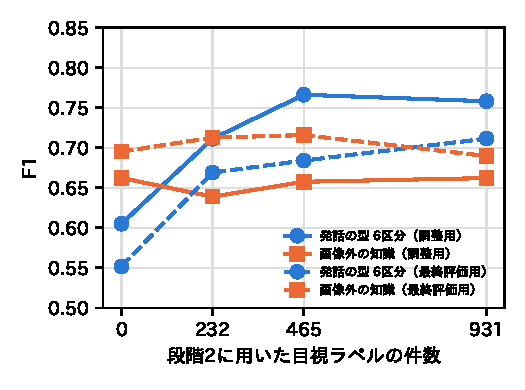
\includegraphics[width=0.95\linewidth]{figures/fig_learning_curve.pdf}
    \caption{段階2に用いた目視ラベルの件数と F1（Qwen3-VL-4B）．0件は段階1のみである．}
    \label{fig_learning_curve}
\end{figure}

最終評価用データの6区分は，232件で0.67，465件で0.68，931件で0.71と，目視ラベルを倍にするごとに0.015〜0.03程度伸びた．
一方，画像外の知識は0.69〜0.72で，目視ラベルの量によらずほぼ一定であった．
931件に検証データの半分（約310件）を加えて残りの半分を予測する2分割の実験でも，6区分は最終評価用で0.71と変わらなかった．
6区分の伸びが続くとしても，0.8に近づけるには数千件以上の目視ラベルが必要と見込まれる．
ただし，これは観測した点からの外挿であり，確かめていない．

\section{画像外の知識の改善の試み}
\label{sec_outside}
発話の型は6区分を信頼性の低いラベルとして扱うことにしたため，以降は画像外の知識の改善に絞った．
本章では，教師ラベルの改善，生徒の構成の変更，ボケの文の再出現の回数の3つの試みを述べる．

\subsection{教師の指示の改善}
教師ラベルの画像外の知識は，学習用の目視ラベル931件との一致が F1 0.59にとどまる．
そこで，32B の教師に画像外の知識だけを問う指示を3つ追加し，目視ラベルのある1,551件で比較した．
追加した指示は，先に元ネタ（作品・人物・台詞・歌詞・CM・流行語・ネットの定型などの引用・もじり・パロディ）を具体的に書かせてから種類・画像内か・必要かを問う指示（src），src に例を加えた指示（src\_fs），src を温度0.7で5回生成して多数決をとる指示（src\_sc）である．

表\ref{tab_outside_teacher}に結果を示す．
元ネタを書き出させると再現率は上がったが，固有名詞や言い回しをなんでも元ネタとみなして「はい」とするため適合率が大きく下がり，F1 はいずれも従来の指示（kt）を下回った．
32B の指示の変更では，教師ラベルを改善できなかった．

\begin{table}[t]
    \centering
    \caption{教師（32B）の画像外の知識の F1．括弧内は学習用931件での適合率と再現率．}
    \label{tab_outside_teacher}
    \small
    \setlength{\tabcolsep}{3pt}
    \begin{tabular}{@{}lccc@{}}
        \toprule
        指示 & 学習用931件 & dev & test \\
        \midrule
        kt（one\_kt\_cap） & \textbf{0.59}（0.54／0.65） & \textbf{0.58} & \textbf{0.67} \\
        src & 0.54（0.44／0.70） & 0.46 & 0.62 \\
        src\_fs & 0.54（0.44／0.68） & 0.55 & 0.64 \\
        src\_sc & 0.54（0.43／0.74） & 0.52 & 0.60 \\
        \bottomrule
    \end{tabular}
\end{table}

\subsection{生徒の構成の変更}
次の要素を変えて，二段階の学習を行った．
\begin{itemize}
    \item モデルの大きさ：InternVL3.5-8B と Qwen3-VL-8B．
    \item 損失の重み：(\ref{eq_loss})の $ \lambda $ を3とする．
    \item 疑似ラベル：段階2まで学習した Qwen3-VL-4B（最終評価用で0.69）で学習用のボケ34,634件の画像外の知識を付け直し，段階1の教師ラベルとする（自己学習\cite{ref_noisy_student}）．
    \item アンサンブル：複数のモデルの画像外の知識の確率の平均．
\end{itemize}
図\ref{fig_outside}と表\ref{tab_outside_student}に結果を示す．

\begin{figure}[t]
    \centering
    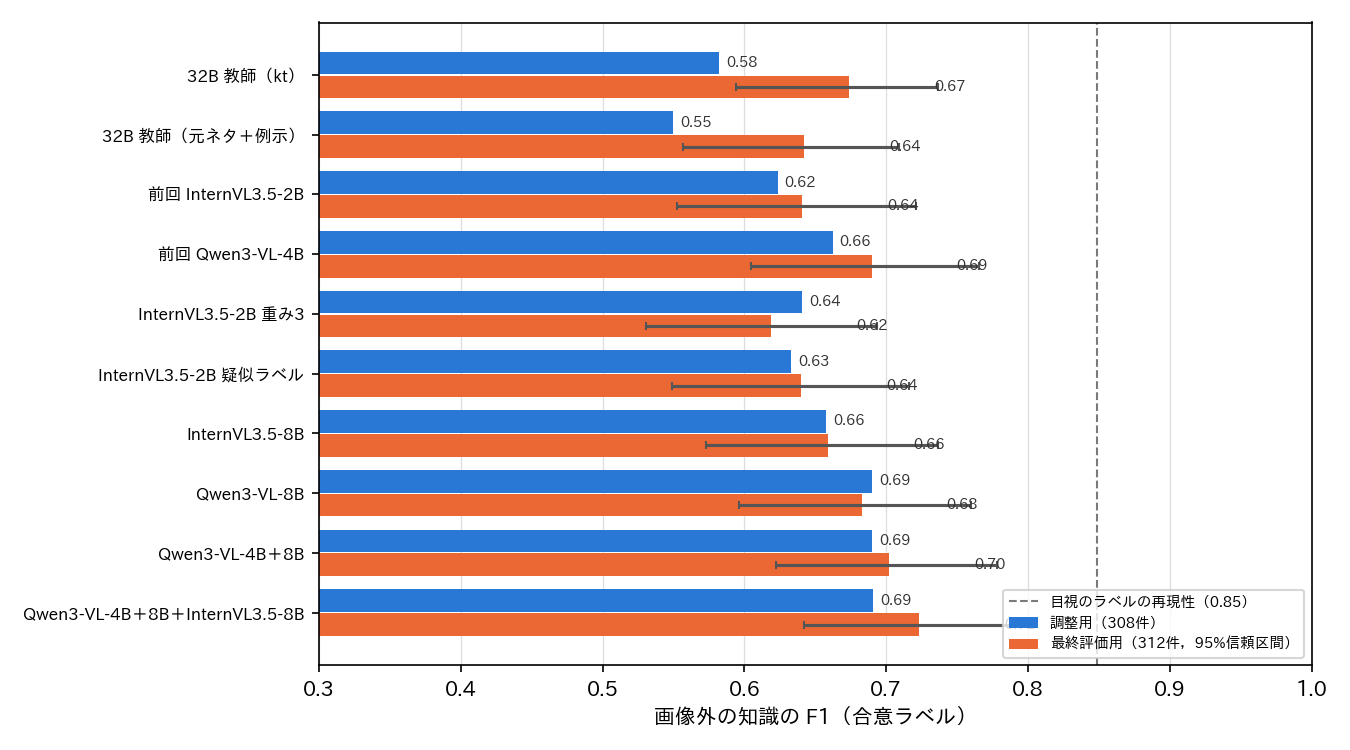
\includegraphics[width=\linewidth]{figures/fig_outside.png}
    \caption{画像外の知識の F1（合意ラベル）．最終評価用は95\%信頼区間を示す．破線は目視ラベルの再現性である．}
    \label{fig_outside}
\end{figure}

\begin{table}[t]
    \centering
    \caption{画像外の知識の改善の試み（段階1＋段階2．AUC は最終評価用）．}
    \label{tab_outside_student}
    \footnotesize
    \setlength{\tabcolsep}{3pt}
    \begin{tabular}{@{}lcccc@{}}
        \toprule
        方法 & dev & test & 95\%区間 & AUC \\
        \midrule
        Qwen3-VL-4B（$\lambda=1$） & 0.66 & 0.69 & 0.60--0.77 & 0.87 \\
        InternVL3.5-2B（$\lambda=1$） & 0.62 & 0.64 & 0.55--0.72 & 0.84 \\
        InternVL3.5-2B（$\lambda=3$） & 0.64 & 0.62 & 0.53--0.69 & 0.83 \\
        InternVL3.5-2B（$\lambda=3$，疑似） & 0.63 & 0.64 & 0.55--0.72 & 0.86 \\
        InternVL3.5-8B（$\lambda=3$） & 0.66 & 0.66 & 0.57--0.74 & 0.85 \\
        Qwen3-VL-8B（$\lambda=3$） & \textbf{0.69} & 0.68 & 0.60--0.76 & 0.85 \\
        Qwen3-VL-4B＋8B & \textbf{0.69} & \textbf{0.70} & 0.62--0.78 & 0.88 \\
        \bottomrule
    \end{tabular}
\end{table}

Qwen3-VL-8B は，調整用で 4B より0.03高かったが，最終評価用ではほぼ同じであった．
InternVL3.5 は 2B から 8B で0.02〜0.04上がったが，Qwen3-VL より低かった．
疑似ラベルは段階1の後では効果があり（最終評価用0.63から0.65），段階2の後では差がなくなった．
損失の重みは効果がなかった．
4B と 8B の確率の平均は，AUC と F1 をわずかに上げた．
いずれの改善も信頼区間の幅（約 $ \pm 0.08 $）より小さく，2〜8B のモデルと教師ラベルの組み合わせでは F1 0.66〜0.70で頭打ちになった．
なお，Qwen3-VL-8B の段階2の後の6区分は，調整用0.76，最終評価用0.74であった．

\subsection{ボケの文の再出現の回数}
有名な台詞や定型を引用するボケは，同じ文が多くのお題に繰り返し投稿されると考えた．
全てのボケの文を正規化（NFKC，小文字化，空白・記号の除去）し，同じ文が投稿されたお題の数を数え，自分のお題を除いた回数を特徴とした．
しかし，この回数の画像外の知識に対する AUC は0.53〜0.56にとどまった．
「なにこれ」「いらっしゃいませ」のような短く一般的な言葉も多くのお題に繰り返し投稿されるためであり，この特徴は用いなかった．

\subsection{誤りの分析}
Qwen3-VL-4B と 8B のアンサンブルの検証データ620件での誤りは，見逃し44件と誤検出51件であった．
表\ref{tab_errors}に例を示す．

\begin{table}[t]
    \centering
    \caption{画像外の知識の誤りの例（Qwen3-VL-4B＋8B）．括弧内は確率．}
    \label{tab_errors}
    \footnotesize
    \begin{tabular}{@{}p{0.16\linewidth}p{0.77\linewidth}@{}}
        \toprule
        種類 & ボケと元ネタ \\
        \midrule
        見逃し & 「バスケがしたいです。」（0.00，漫画の名台詞） \\
        & 「返事がない。ただの壁のようだ。」（0.02，ゲームの定型文のもじり） \\
        & 「俺か俺以外か」（0.00，タレントの決め台詞） \\
        & 「こうかはいまひとつのようだ」（0.10，ゲームの定型文） \\
        \midrule
        誤検出 & 「ジャムおじさんを基準にすると巨人の星」（1.00，画像は同じ作品） \\
        & 「くまモンに丸のみされたなっしー・・・。」（1.00） \\
        & 「だるまさんがこーろんだっ！」（0.99，一般の遊び） \\
        \bottomrule
    \end{tabular}
\end{table}

見逃しの大半は，有名な台詞・歌詞・ネットの定型の引用であった．
例えば，漫画の名台詞を借りた「バスケがしたいです。」，ゲームの定型文をもじった「返事がない。ただの壁のようだ。」，タレントの決め台詞である「俺か俺以外か」であり，字面は普通の日本語であるため，元ネタを知らないモデルには判定できない．
誤検出の多くは，画像に写っている作品の登場人物を画像外とするものであった．
例えば，アンパンマンの画像に対する「ジャムおじさん」や「バタコさん」を含むボケである．
また，固有名詞を含むだけで一般の知識で面白さが分かるボケも誤検出された．
見逃しは知識の量の問題であり，2〜8B のモデルの微調整では改善が限られる．
誤検出は画像に写っている作品の同定の問題であり，お題画像ごとに写っている作品を同定して入力に加えることで改善できる可能性がある．

\section{推論の高速化}
\label{sec_speed}
\subsection{プレフィックスの共有}
\ref{sec_vlm}章の分類器は，ボケ1件ごとに，お題画像のトークンとお題の文を含む約300トークンを計算する．
しかし，同じお題のボケ（平均約14件）では，入力の「ボケ：「」までの部分（プレフィックス）が共通である．
そこで，図\ref{fig_prefix}のように計算を分けた．

\begin{figure}[t]
    \centering
    \begin{tikzpicture}[font=\scriptsize, node distance=3mm,
        box/.style={draw, rounded corners=2pt, minimum height=5mm, align=center, inner sep=2pt}]
        \node[box, fill=gray!15, minimum width=34mm] (pre) {お題画像＋お題の文（プレフィックス）\\ 約250〜300トークン，お題ごとに1回};
        \node[box, below=4mm of pre, minimum width=34mm] (kv) {KV キャッシュ};
        \node[box, below left=5mm and -12mm of kv, minimum width=14mm] (s1) {ボケ1};
        \node[box, right=2mm of s1, minimum width=14mm] (s2) {ボケ2};
        \node[right=1mm of s2] (dots) {$\cdots$};
        \node[box, right=1mm of dots, minimum width=14mm] (sn) {ボケ $ n $};
        \node[box, below=4mm of s2, minimum width=50mm] (head) {最後のトークンの隠れ状態 $\rightarrow$ (\ref{eq_heads})};
        \draw[-{Stealth}] (pre) -- (kv);
        \draw[-{Stealth}] (kv) -- (s1);
        \draw[-{Stealth}] (kv) -- (s2);
        \draw[-{Stealth}] (kv) -- (sn);
        \draw[-{Stealth}] (s1) -- (head);
        \draw[-{Stealth}] (s2) -- (head);
        \draw[-{Stealth}] (sn) -- (head);
    \end{tikzpicture}
    \caption{プレフィックスの共有による推論．お題ごとにプレフィックスを1回計算して KV キャッシュを作り，ボケの数だけ複製して，ボケの文と閉じ括弧以降（約20〜60トークン）だけを計算する．}
    \label{fig_prefix}
\end{figure}

お題 $ g $ のボケの数を $ n_g $，プレフィックスの長さを $ L_{\rm p} $，ボケ $ i $ の部分の長さを $ L_{i} $ とすると，計算するトークン数は(\ref{eq_tokens})のように減る．

\begin{equation}
    \sum_{g} \sum_{i=1}^{n_g} ( L_{\rm p} + L_{i} ) \; \rightarrow \; \sum_{g} \left( L_{\rm p} + \sum_{i=1}^{n_g} L_{i} \right)
    \label{eq_tokens}
\end{equation}

\noindent
例えば $ n_g = 14 $，$ L_{\rm p} = 270 $，$ L_{i} = 40 $ とすると，計算するトークン数は約1/5になる．
InternVL3.5 は画像のトークン数が一定であるため，プレフィックスの長さが同じお題をまとめて計算した．
Qwen3-VL は画像ごとにトークン数が異なり，位置が3次元の回転位置埋め込みであるため，プレフィックスを左詰めでまとめて計算し，ボケの部分の位置はプレフィックスの最大の位置の次から続けた．
プレフィックスとボケの部分は別々にトークン化するため，境界のトークン化が通常の推論とわずかに異なる場合がある．

\subsection{結果}
検証データ620件で通常の推論と比べると，判定の一致は InternVL3.5-2B で99.7\%，Qwen3-VL-4B で99.8\%，画像外の知識の確率の差の平均は0.003であった．
速度は，データベースから無作為に選んだ600件のお題の全てのボケ（8,664件，1お題あたり14.4件）を，画像の読み込みと前処理を含めて処理して測った．
GPU は RTX PRO 6000（96GB）1枚，前処理は8プロセスである．
図\ref{fig_speed}に結果を示す．

\begin{figure}[t]
    \centering
    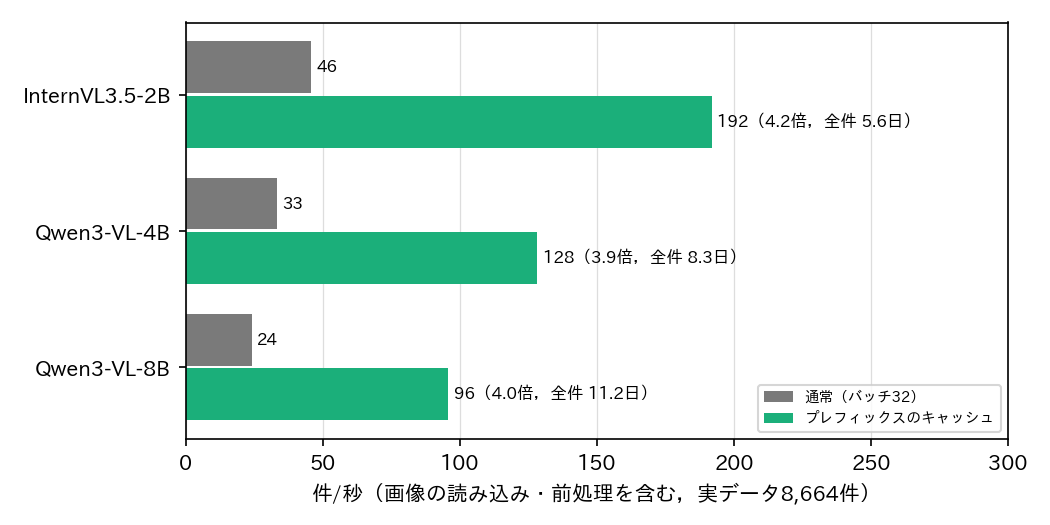
\includegraphics[width=\linewidth]{figures/fig_speed.png}
    \caption{通常の推論（バッチ32）とプレフィックスの共有による推論の1秒あたりの件数．括弧内は倍率と，約9,250万件の推定処理日数である．}
    \label{fig_speed}
\end{figure}

プレフィックスの共有により，InternVL3.5-2B は46件/秒から192件/秒，Qwen3-VL-4B は33件/秒から128件/秒，Qwen3-VL-8B は24件/秒から96件/秒となり，いずれも約4倍に高速化した．
全件の推定処理時間は，Qwen3-VL-4B で約32日から約8.3日，Qwen3-VL-8B で約11日となった．
一度にまとめるボケを1,024件に増やすと GPU のメモリの圧迫で遅くなり，256〜512件が最適であった．
前処理のプロセスを16に増やしても速くならなかったため，GPU の計算が律速である．

表\ref{tab_time}に，本稿で扱った主な方法で全件を処理する場合の推定時間をまとめる．
VLM の教師を全件に適用するには数か月から1年近くを要し，現実的ではない．
文の生徒は数時間で処理できるが，画像外の知識の精度が低い．
プレフィックスを共有した小さな VLM は，精度と処理時間の両方で実用的な範囲にある．

\begin{table}[t]
    \centering
    \caption{約9,250万件の処理時間の見積もり（単一の GPU）．F1 は最終評価用（合意ラベル）．}
    \label{tab_time}
    \footnotesize
    \setlength{\tabcolsep}{2.5pt}
    \begin{tabular}{@{}lcccr@{}}
        \toprule
        方法 & 件/秒 & 6区分 & 画像外 & 全件 \\
        \midrule
        教師 32B（one\_kt\_cap） & 3.9 & 0.56 & 0.67 & 約270日 \\
        文の生徒 & --- & 0.61 & 0.60 & 数時間 \\
        Qwen3-VL-4B（通常） & 33 & 0.71 & 0.69 & 約32日 \\
        InternVL3.5-2B（共有） & 192 & 0.71 & 0.64 & 約5.6日 \\
        Qwen3-VL-4B（共有） & 128 & 0.71 & 0.69 & 約8.3日 \\
        Qwen3-VL-8B（共有） & 96 & 0.74 & 0.68 & 約11日 \\
        Qwen3-VL-4B＋8B（共有） & 55 & 0.71 & 0.70 & 約19日 \\
        \bottomrule
    \end{tabular}
\end{table}

\section{考察}
\label{sec_discussion}
\subsection{ラベルの定義と精度の上限}
本研究で最も大きな影響を持ったのは，ラベルの定義であった．
必要な知識の4段階は，目視では上から順に判定でき，判断の手順として妥当であったが，自動判定のマクロ F1 は0.48を超えなかった．
2値に改めて条件を厳密にしたことで，教師の画像外の知識は F1 0.32から0.67に上がった．
これは主に，指示に依存する事物の種類を選ばせ，普通名詞を特定の事物とする誤りを抑えたことによる．
また，付け直しによる再現性の測定は，同じ判断者でも6区分の約14\%，画像外の知識の約7\%の判断が揺れ，F1 ではそれぞれ0.80と0.85にとどまることを示した．
自動判定の目標値を決める前に，この上限を測っておくことが重要である．
一方で，この上限は同一の判断者の再現性であり，複数の判断者の間の一致度はさらに低い可能性がある．

\subsection{教師の偏りと少量の目視ラベル}
VLM の教師は，セリフをツッコミとし，状況の説明をほとんど使わず，一般的な語を特定の事物とするといった系統的な偏りを持っていた．
蒸留した生徒はこの偏りを受け継ぐため，教師ラベルだけでは教師の水準を超えにくい．
指示の分解や例示による偏りの修正は，かえって別の偏りを生んだ．
これに対し，931件の目視ラベルによる微調整は，6区分を0.55から0.71に上げた．
大量の教師ラベルで画像外の知識に必要な表現を学び，少量の目視ラベルで区分の境界を学ぶ二段階の学習は，教師の偏りを直接直すより効率的であった．
ただし，目視ラベルを増やす効果は緩やかであり，6区分で0.8に近づけるには，目視ラベルを大きく増やすか，揺れの大きいツッコミと心の声の定義を見直す必要がある．

\subsection{画像外の知識の限界}
画像外の知識の見逃しの多くは，有名な台詞や定型の引用に気づかないことによる．
字面が普通の日本語である引用は，元ネタを知らなければ判定できず，2〜8B のモデルの持つ知識では限界がある．
32B の教師も元ネタを書き出させると過剰に「はい」とし，教師ラベルの改善には結びつかなかった．
より大きなモデルを目視ラベルで微調整して教師とすることや，お題画像ごとに写っている作品を一度だけ同定して入力に加えることが，次の候補である．
後者はお題ごとに1回の処理であり，\ref{sec_speed}章のプレフィックスの共有とも両立する．

\subsection{本研究の限界}
本研究の目視ラベルは，全て AI エージェントである Claude Code が付与したものであり，人の判断者によるラベルとの一致は測っていない．
大喜利の解釈には文化的な知識や感覚が関わるため，人の判断者による検証が必要である．
また，検証データは620件であり，最終評価用データの F1 の95\%信頼区間は約 $ \pm 0.08 $ と広い．
本稿で比較した多くの改善は，この幅より小さい．
さらに，本稿の方法はまだ全件には適用しておらず，全件のラベルの分布や，下流の生成・判定での有用性は検証していない．

\section{おわりに}
\label{sec_conclusion}
本稿では，大喜利投稿サイト「ボケて」の約9,250万件のボケに，構造を表すラベルを付与する方法を検討した経緯を報告した．
実例の読解から，制約の順守，発話の型，画像外の知識の3つの観点を定め，定義書を3回改訂した．
検証データ620件の付け直しにより，発話の型の6区分で F1 0.80，画像外の知識で0.85という目視ラベルの再現性を示し，これを自動判定の実質的な上限とした．
制約の順守は，カルタでは書き出しの規則で，穴埋めとお題文では同じお題の他のボケとの類似度で判定できることを示した．
発話の型と画像外の知識については，お題画像とボケを入力とする小さな VLM を，教師ラベルで学習した後に少量の目視ラベルで微調整する二段階の学習が最も有効であり，最終評価用データで6区分のマクロ F1 0.71〜0.74，3区分0.86〜0.88，画像外の知識の F1 0.68〜0.70を得た．
さらに，同じお題のボケでプレフィックスの計算を共有することで，推論を約4倍に高速化し，Qwen3-VL-4B で全件を約8日で処理できる見込みを得た．

今後は，人の判断者によるラベルで目視ラベルの妥当性を確かめるとともに，ツッコミと心の声の定義を見直す．
また，画像に写っている作品の同定と，より大きなモデルによる教師ラベルの改善により，画像外の知識の判定を改善する．
そのうえで，全件にラベルを付与し，大喜利の生成と判定の研究に用いる．


\vspace{-1mm}
\begin{thebibliography}{99}

    \bibitem{ref_oogiri_go}
    S. Zhong, et al., ``Let's Think Outside the Box: Exploring Leap-of-Thought in Large Language Models with Creative Humor Generation,'' Proc. CVPR, 2024.

    \bibitem{ref_newyorker}
    J. Hessel, et al., ``Do Androids Laugh at Electric Sheep? Humor ``Understanding'' Benchmarks from The New Yorker Caption Contest,'' Proc. ACL, 2023.

    \bibitem{ref_bokete}
    ボケて (bokete), https://bokete.jp/, (2026年10月閲覧).

    \bibitem{ref_qwen3vl}
    Qwen Team, ``Qwen3-VL Technical Report,'' arXiv:2511.21631, 2025.

    \bibitem{ref_internvl35}
    W. Wang, et al., ``InternVL3.5: Advancing Open-Source Multimodal Models in Versatility, Reasoning, and Efficiency,'' arXiv:2508.18265, 2025.

    \bibitem{ref_gemma3}
    Gemma Team, ``Gemma 3 Technical Report,'' arXiv:2503.19786, 2025.

    \bibitem{ref_smolvlm}
    A. Marafioti, et al., ``SmolVLM: Redefining Small and Efficient Multimodal Models,'' arXiv:2504.05299, 2025.

    \bibitem{ref_lfm2vl}
    Liquid AI, ``LFM2-VL,'' https://huggingface.co/LiquidAI/LFM2-VL-1.6B, (2026年10月閲覧).

    \bibitem{ref_vllm}
    W. Kwon, et al., ``Efficient Memory Management for Large Language Model Serving with PagedAttention,'' Proc. SOSP, 2023.

    \bibitem{ref_sglang}
    L. Zheng, et al., ``SGLang: Efficient Execution of Structured Language Model Programs,'' Proc. NeurIPS, 2024.

    \bibitem{ref_kd}
    G. Hinton, O. Vinyals, and J. Dean, ``Distilling the Knowledge in a Neural Network,'' arXiv:1503.02531, 2015.

    \bibitem{ref_noisy_student}
    Q. Xie, M.-T. Luong, E. Hovy, and Q. V. Le, ``Self-Training with Noisy Student Improves ImageNet Classification,'' Proc. CVPR, 2020.

    \bibitem{ref_lora}
    E. J. Hu, et al., ``LoRA: Low-Rank Adaptation of Large Language Models,'' Proc. ICLR, 2022.

    \bibitem{ref_ruri}
    H. Tsukagoshi and R. Sasano, ``Ruri: Japanese General Text Embeddings,'' arXiv:2409.07737, 2024.

    \bibitem{ref_me5}
    L. Wang, et al., ``Multilingual E5 Text Embeddings: A Technical Report,'' arXiv:2402.05672, 2024.

    \bibitem{ref_kappa}
    J. Cohen, ``A Coefficient of Agreement for Nominal Scales,'' Educational and Psychological Measurement, vol. 20, no. 1, pp. 37--46, 1960.

    \bibitem{ref_adamw}
    I. Loshchilov and F. Hutter, ``Decoupled Weight Decay Regularization,'' Proc. ICLR, 2019.

\end{thebibliography}


\end{document}
